\chapter{Slope-induced tidal straining: Analysis of rotational effects}
\label{kap-jgr}

Tidal straining is known to be an important factor for the generation
of residual currents and transports of suspended matter in the coastal
ocean. Recent modeling studies and field experiments have revealed a
new type of ``slope-induced'' tidal straining, in which the horizontal
density gradient required for this process is induced by the presence
of a slope rather than by river runoff (as in classical tidal
straining). Slope-induced tidal straining is investigated here with
the help of an idealized numerical model, and results are compared to
a recent data set from the East China Sea providing first direct
observational evidence. The focus of this study is on the effect of
rotation that was ignored in previous investigations. The model is
shown to reproduce the key features of the observations, in particular
the strain-induced generation of unstable stratification in the bottom
boundary layer during periods of upslope flow. Rotation effects are
found to significantly reduce the upslope tidal pumping of suspended
material but also give rise to a newly identified pumping mechanism
that results in a vigorous transport of suspended material along the
slope. It is shown that slope-induced tidal straining is likely to be
relevant for a wide range of oceanic slopes exposed to tidal motions.

\section{Introduction}
In many estuaries and regions of the coastal ocean, the tidal dynamics
and the generation of residual transports are strongly modified by the
presence of a horizontal density gradient, typically maintained by
river runoff or differential heating. In these cases, the horizontal
density gradient interacts with the vertical tidal shear to induce a
periodic modulation of the vertical density structure that is usually
referred to as Strain-Induced Periodic Stratification (SIPS). During
flood, dense water is advected on top of lighter water, thus
destabilizing the water column, whereas during ebb, light water is
transported on top of denser water, inducing stable stratification
\citep{vanAken86a,Simpsonetal90a}.

\cite{MacCreadyGeyer2014a} summarized the present understanding of the
dynamical implications of this tidal straining process, highlighting
in particular the role of SIPS for the generation of tidal asymmetries
in mixing (see their Fig.\ 2). They pointed out that the generally
larger turbulent diffusivities observed during the less stratified
flood phase are reflected in tidal asymmetries in the velocity
profiles, inducing a landward residual circulation near the bottom,
and a seaward return current in the upper part of the water
column. From extensive numerical experiments,
\cite{BurchardHetland2010a} concluded that in tidally energetic systems
the contribution of this ``tidal straining circulation'' to the total
residual circulation may be significantly larger than the
gravitationally-driven component, challenging the classical view of
estuarine circulation.

\cite{JayMusiak94a} proposed that the mixing asymmetries due to SIPS
may also have a profound impact on the residual transport of suspended
material. These authors showed that due to stronger turbulence during
the flood phase, high concentrations of suspended material are
generally correlated with flood currents (directed landward), thus
inducing a residual landward transport of suspended material
\citep{Unclesetal85a,JayMusiak94a,ScullyFriedrichs2007a}. Idealized
numerical experiments revealed that this ``tidal pumping'' mechanism
generally dominates over the advection of suspended material by the
residual current \citep{Burchardetal2013a}. 

\begin{figure}
  \noindent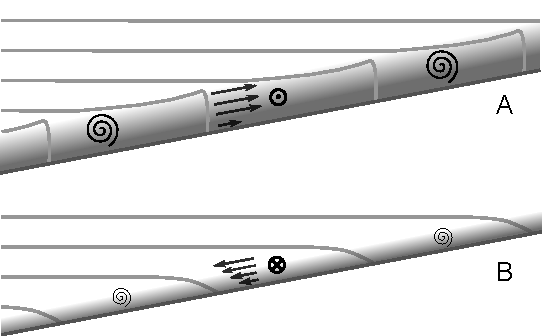
\includegraphics[width=30pc]{sketch.pdf}
  \caption{Slope-induced tidal straining causing (a) unstable
    stratification during upslope flow and (b) stable stratification
    during downslope flow (SIPS). Gray lines denote isopycnals, arrows
    show the current direction. Gray-shaded areas near the bottom
    indicate the presence of suspended material; spirals symbolize
    near-bottom turbulence.}
  \label{sketch}
\end{figure}

In a recent modeling study, \cite{schulzumlauf2016} proposed that
similar tidal straining and pumping processes may occur also in
vicinity of a topographic slope --- with the important difference,
however, that no externally imposed horizontal density gradient (e.g.,
due to river runoff) is required. In this case, the (quasi-)horizontal
density gradient is generated by the projection of the vertical
interior density gradient onto the slope
(Fig.\ \ref{sketch}). Slope-induced tidal straining is confined to a
turbulent bottom boundary layer (BBL), but the process is otherwise
completely analogous to classical tidal straining over a flat bottom:
during upslope flow, dense water is advected on top of lighter water,
resulting in unstable stratification, enhanced near-bottom turbulence,
and high concentrations of suspended material
(Fig.\ \ref{sketch}a). Vice-versa, during downslope flow, the
straining of the cross-slope density gradient induces a tendency for
increasing stratification inside the BBL, which in turn leads to
reduced BBL turbulence, smaller BBL thicknesses, and lower sediment
concentrations. Using an idealized one-dimensional (slope-normal)
numerical model, \cite{schulzumlauf2016} showed that tidal pumping
leads to a net cross-slope transport of suspended material, similar to
the tidal pumping mechanism over a flat bottom described by
\cite{JayMusiak94a}. In their study, \cite{schulzumlauf2016} ignored
the effect of rotation, which may, however, be essential in many
realistic settings. This point will therefore be investigated in
detail in the following analysis.

First observational evidence for slope-induced tidal straining was
recently discussed by \cite{Endohetal2016a}, who analyzed an extensive
data set, including turbulence microstructure observations, from a
topographic slope exposed to strong tidal currents in the East China
Sea. These authors described a periodic destabilization of the water
column during periods with upslope tidal currents, induced by the
presence of a persistent cross-slope density gradient. The latter
turned out to be consistent with the projection of the vertical
density gradient onto the slope, and therefore with the importance of
slope-induced tidal straining.

Here, we attempt to clarify the mechanisms, implications, and
relevance of slope-induced tidal straining on a real oceanic shelf by
combining the results from previous modeling studies by
\cite{UmlaufBurchard2011a} and \cite{schulzumlauf2016} with the
experimental data by \cite{Endohetal2016a}.  In section
\ref{modeldescription}, we extend the model used by
\cite{schulzumlauf2016} to include the effects of rotation before we
briefly summarize the field observations discussed by
\cite{Endohetal2016a} in section \ref{studysite}. After deriving model
parameters from these observations in section \ref{observations}, we
discuss the model results in section \ref{modelresults}, and compare
them to the field data. The implications of tidal straining for the
generation of residual currents and the residual transport of
suspended material are analyzed in section \ref{residuals} before we
draw some conclusions in section \ref{conclusions}.


\section{Model description}\label{modeldescription}

\subsection{Model geometry}\label{modelgeometry}

\begin{figure}
  \noindent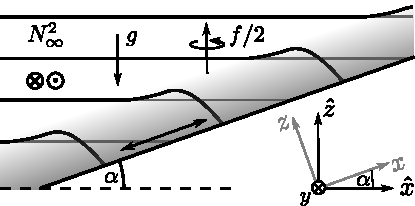
\includegraphics[width=30pc]{geometry.pdf}
  \caption{Schematic view of the model geometry and density structure
    (black lines) near a uniform slope with slope angle $\alpha$. Gray
    lines indicate isopycnal equilibrium levels ($b_\infty =
    const.$). Upslope and slope-normal coordinates are denoted by $x$
    and $z$, respectively. Arrows symbolize the oscillating
    near-bottom currents.}
  \label{geometry}
\end{figure}

Following previous modeling studies of slope-induced straining
\citep{UmlaufBurchard2011a,schulzumlauf2016}, we investigate in the
following the motion of a vertically stratified Boussinesq fluid in
the vicinity of a uniform slope with slope angle $\alpha$. The
geometry is two-dimensional with the horizontal and vertical
coordinates denoted by $\hat{x}$ and $\hat{z}$, respectively, and the
fluid is assumed to rotate with angular velocity $f / 2$ about the
vertical axes (Fig.\ \ref{geometry}). Vertical stratification is
quantified with the help of the buoyancy frequency,
\begin{equation}
  \label{N2}
  N^2 = \frac{\partial b}{\partial \hat{z}} \, ,
\end{equation}
where $b$ denotes buoyancy. Above the BBL, we assume that isopycnals
remain strictly horizontal during all times, and that $N^2$ approaches
the constant background value $N^2_\infty$. Close to the bottom,
however, isopycnals will be distorted as a result of boundary mixing,
and the local buoyancy $b$ will differ from the equilibrium buoyancy
$b_\infty$ (black and gray lines Fig.\ \ref{geometry}).

Introducing a rotated coordinate system with the cross-slope,
along-slope, and slope-normal coordinates denoted by $x$, $y$, and $z$
(see Fig.\ \ref{geometry}), it can be shown from simple geometrical
arguments that under the above conditions also the cross-slope
buoyancy gradient is constant:
\begin{equation}
  \label{dbdx}
  \frac{\partial b}{\partial x} = N^2_\infty \sin \alpha \, ,
\end{equation}
illustrating the generation of a quasi-horizontal ($\alpha \ll 1$)
buoyancy gradient by the projection of the purely vertical interior
stratification onto the slope
\citep{Garrettetal93a,UmlaufBurchard2011a}.

\subsection{Model equations}\label{modelequations}

Assuming that all cross-slope and along-slope gradients vanish, except
the cross-slope buoyancy gradient defined in (\ref{dbdx}), the problem
becomes geometrically one-dimensional in the slope-normal
$z$-direction. The Boussinesq equations can then be written as
\citep{Umlaufetal2015a}:
\begin{align}
  \label{ueq}
  \frac{\partial u}{ \partial t} -fv \cos \alpha  &= (b - b_\infty) \sin \alpha 
+ P_x - \frac{\partial \tau_x}{ \partial z} \, , \\
  \label{veq}
  \frac{ \partial v}{\partial t} + fu \cos \alpha &= P_y - 
\frac{\partial \tau_y}{\partial z}                             \, , \\
  \label{beq}  
  \frac{\partial b}{\partial t} &= -u N^2_\infty \sin \alpha - 
\frac{\partial G}{\partial z}                              \, , 
\end{align}
with $u$ and $v$ denoting the upslope and along-slope velocities, and
$\tau_x$, $\tau_y$ and $G$ the slope-normal turbulent fluxes of
momentum (per unit mass) and buoyancy, respectively. $P_x(t)$ and
$P_y(t)$ are integration constants that play the role of prescribed
external pressure gradients. The cross-slope buoyancy gradient in the
advection term in (\ref{beq}) has been expressed with the help of
(\ref{dbdx}). Note that in contrast to previous studies of
slope-induced tidal straining that only considered the plane
non-rotating case ($f=0$, $v=0$), equations (\ref{ueq}) -- (\ref {beq}) now
include rotational effects that turned out to be essential to describe
the motions at our study site.

The equilibrium buoyancy $b_\infty$ appearing in the first term on the
right hand side of (\ref{ueq}) evolves as a result of cross-slope
buoyancy advection, and can therefore be described by an advection
equation of the form.
\begin{equation}
  \label{binf}
  \frac{\partial b_\infty}{\partial t} + u_\infty N_\infty^2 \sin \alpha = 0 \, 
,
\end{equation}
which directly follows from (\ref{beq}) for $z \rightarrow \infty$.

Far away from the boundary ($z\rightarrow \infty$), we assume that all
slope-normal gradients, except the buoyancy gradient vanish, whereas at
the lower boundary ($z = 0$) we use the boundary conditions
\begin{equation}
  \label{uvbBC}
  u=v=0, \quad \frac{\partial b}{\partial z}=0 \, .
\end{equation}

\cite{schulzumlauf2016} also discussed a simple transport equation for
the concentration $c$ of suspended particulate material (SPM)
exhibiting a vertical sinking motion $w_s$ relative to the moving
fluid:
\begin{equation}
  \label{ceq}
  \frac{\partial c}{\partial t} = - \frac{\partial }{\partial z} \left( F_z - c 
w_s  \cos \alpha \right) \, , 
\end{equation}
where $F_z$ is the slope-normal turbulent SPM flux. At the bottom,
this flux equals the erosion flux:
\begin{equation}
  \label{Fz}
  F_z = \alpha_e \max \left\{ \frac{|\tau_b|}{\tau_c} -1,0 \right\} \quad 
\text{at $z=0$} \, ,
\end{equation}
where $\alpha_e$ is the erosion parameter, $\tau_b$ the bottom stress,
and $\tau_c$ the critical shear stress for erosion.

The turbulent fluxes appearing in (\ref{ueq}) -- (\ref{beq}) and
(\ref{ceq}) are computed from gradient expressions of the form
\begin{equation}
  \label{turbfluxes}
  \tau_x = - \nu_t   \frac{\partial u}{\partial z} \, , \quad
  \tau_y = - \nu_t   \frac{\partial v}{\partial z} \, , \quad
  G      = - \nu^b_t \frac{\partial b}{\partial z} \, , \quad
  F_z    = - \nu^b_t \frac{\partial c}{\partial z} \, , 
\end{equation}
where $\nu_t$ is the turbulent viscosity, and $\nu^b_t$ the turbulent
diffusivity of buoyancy and SPM. The diffusivities are computed from a
second-moment turbulence model that includes two prognostic equations
for the turbulent kinetic energy $k$ and the dissipation rate
$\varepsilon$. This turbulence model is identical to that described in
detail in \cite{UmlaufBurchard2011a}, \cite{Umlaufetal2015a}, and
\cite{schulzumlauf2016}, and, for brevity, this description is not
repeated here. The general properties of this class of turbulence
models are reviewed in \cite{UmlaufBurchard2005a}; details about the
numerical implementation may be found in \cite{Umlaufetal2005a}. In
the non-turbulent region above the BBL ($z \rightarrow \infty$), the
turbulent fluxes are assumed to vanish.  Also, as we only investigate
flows at high Reynolds number in this study, all molecular fluxes are
ignored.

\subsection{Model properties}\label{modelproperties}
In the following, we will assume that BBL motions are driven by a
harmonic horizontal pressure force pointing into an arbitrary
horizontal direction, here referred to as the $n$-direction:
\begin{equation}
  \label{Pn}
  P_n = P \cos (\omega t + \phi) \; ,
\end{equation}
where $\omega$ is the forcing frequency, $\phi$ the phase, and $P$ the
magnitude of the pressure force. Denoting the angle between the $n$-
and $x$-directions as $\beta$, the components of $P_n$ in the $x$- and
$y$-directions are $P_x = P_n \cos \beta$ and $P_y = P_n \sin
\beta$. It is straightforward to show from (\ref{ueq}) and (\ref{veq})
that for the harmonic forcing in (\ref{Pn}), the velocities in the
inviscid region above the BBL ($z\rightarrow \infty$) are described by
\begin{align}
  \label{Un}
  u_n & = P \frac{\omega}{\omega^2 - f^2} \sin ( \omega t + \phi) \\
  u_s & = P \frac{f     }{\omega^2 - f^2} \cos ( \omega t + \phi) \, ,
  \label{Us}
\end{align}
with $u_n$ and $u_s$ denoting the components in the $n$- and
$s$-directions, respectively (the latter obtained from rotating the
$y$-axis by the angle $\beta$). For $\omega>f$, the velocity vector is
seen to anti-cyclonically trace an ellipse with axes ratio
$e=\omega/f$, where the main axis points into the direction of the
pressure gradient. Due to the lack of viscous damping in the
non-turbulent layer above the BBL, velocities increase toward infinity
if resonance is reached ($\omega=f$). The harmonic pressure term in
(\ref{Pn}) will be used below as a simple representation of tidal
forcing in a rotating system

The situation becomes more complex inside the BBL due to the
appearance of the internal pressure term $(b-b_\infty) \sin \alpha$ in
(\ref{ueq}). \cite{Umlaufetal2015a} showed that this term represents
the tendency of isopycnals to relax back to their equilibrium
positions ($b=b_\infty$), which implies the possibility of reversible
BBL oscillations at the frequency
\begin{equation}
  \label{omegac}
  \omega_c^2 = f^2 \cos^2 \alpha + N_\infty^2 \sin^2 \alpha \, ,
\end{equation}
indicating that BBL resonance occurs for $\omega=\omega_c$
\citep{UmlaufBurchard2011a}. Vice-versa, if $N_\infty$, $f$, and
$\omega$ are considered to be given, BBL resonance will be observed if
the slope $\alpha$ approaches the critical slope $\alpha_c$ found from
inverting (\ref{omegac}). Model properties exhibit qualitative changes
during the transition from subcritical to supercritical slopes, and
some of the model assumptions break down near critical slopes
\citep{UmlaufBurchard2011a,schulzumlauf2016}.

Near the geographic location investigated in this study, the
parameters $N^2_\infty,\, f,$ and $\alpha$ are derived in the chapters
below and summarized in Tab.\ \ref{input}. The frequency for critical
boundary layer resonance derived from these parameters is $\omega_c =
7.69 \times 10^{-5}$~s~$^{-1}$, corresponding to a period of $T_c = 22.7$~h. As
discussed in more detail below, the proximity of $T_c$ to the diurnal
tidal period is one of the reason why the diurnal tides are neglected
in our model analysis.

\begin{table}
\caption{Standard parameters used for the simulations in sections
  \ref{modelresults} and \ref{residuals}}\label{input}
\begin{center}
\begin{tabular}{ccccccc}
\hline
\hline
$\alpha$ & $N_\infty^2$ & $f$ & $z_0$ & $\tau_c$ & $\alpha_e$ \\
\hline
$3 \times 10^{-4}$ & $6.5 \times 10^{-4}\, \text{s}^{-2}$ & $7.65 \times 
10^{-5}\, 
\text{s}^{-1}$ & $10^{-3}\, \text{m}$ & $10^{-4}$~m$^2$~s$^{-2}$ & 
$10^{-4}$~kg~s$^{-1}$~m$^{-2}$ \\
\hline
\end{tabular}
\end{center}
\end{table}

Finally, for the following discussion of residual transports it is
useful to note that \cite{UmlaufBurchard2011a} showed that under the
above conditions (harmonic forcing, zero mixing above the BBL), the
residual upslope transport vanishes
\begin{equation}
  \label{uint}
  \int_0^\infty \langle u \rangle dz = 0 \, ,
\end{equation}
where the angular brackets denote the average over one forcing period
$T = 2 \pi / \omega$.

\section{Study site and methods}\label{methods}

\subsection{Study site}

\begin{figure}
  \noindent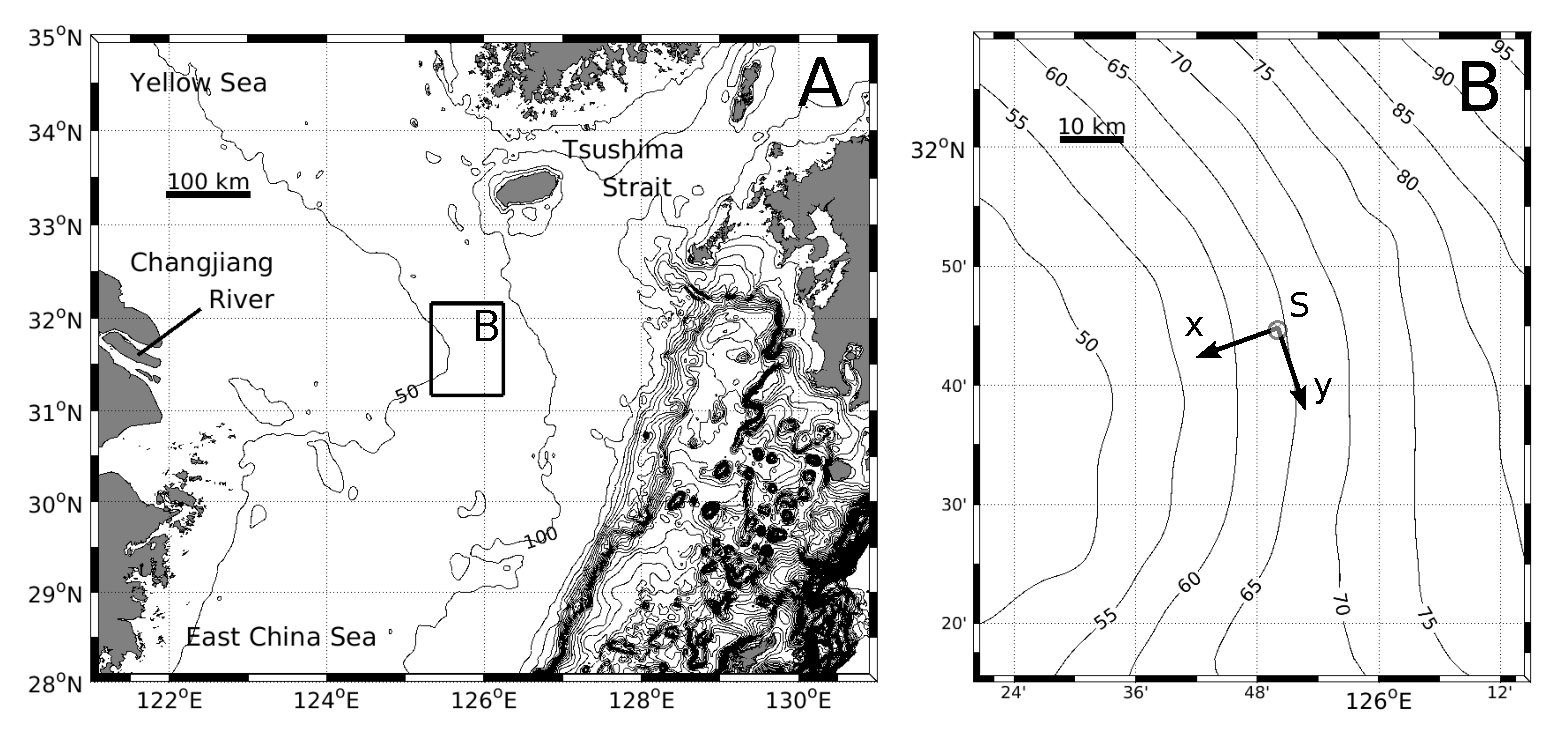
\includegraphics[width=40pc]{studyside.pdf}
  \caption{Maps of (a) East China Sea, and (b) study area with
    deployment location ``S''. Local cross-slope and along-slope
    directions are denoted by $x$ and $y$ (rotated by 20 degrees with
    respect to the zonal and meridional directions,
    respectively). Bathymetry is in meters, based on bathymetric data
    described in \cite{Choietal2002a}.}
  \label{studysite}
\end{figure}

In July 2011, hydrographic and turbulence microstructure measurements
were performed near position S in the East China Sea
(Fig.\ \ref{studysite}). The study site was located at $31^\circ
44.9'\,\text{N}, \, 125^\circ 50.0'\,\text{E}$ on a mildly sloping
continental shelf at approximately 68~m water depth. The inertial
period at this latitude is $T_f = 23.3$ hours. Based on a
finite-element global ocean tidal model with a regionally refined
numerical grid, \cite{Lefevreetal2000} showed that the East China Sea
is subject of strong tidal motions with the four major constituents
being: the principal lunar and solar tides, $M_2$ and $S_2$, with
semi-diurnal periods, and the luni-solar and principal lunar diurnal
tides, $K_1$ and $O_1$, respectively. The $M_2$ tide is dominant here,
about three times stronger than the second largest tidal component,
the $S_2$. The two diurnal tides are of similar magnitude and about 4
times weaker than the $M_2$ component. Similar results were derived from 
observations of current velocity data at  $31^\circ 45'\,\text{N}, \, 127^\circ 
25'\,\text{E}$ (east of position S) \citep[][]{Yoshikawaetal2012a}. It should 
be noted that the inertial period is close to the periods of the diurnal tides,
precluding a straightforward spectral distinction between diurnal
tidal and near-inertial signals in a short time series.

Fig.\ \ref{studysite} illustrates that position S is located
approximately 400~km away from the Changjiang river mouth, which forms
the by far largest freshwater source in this
region. \cite{Endohetal2016a} pointed out that this large spatial
separation, and the fact that the less dense river water will mainly
affect the near-surface layer during the thermally stratified summer
period, suggests that the BBL at position S is unlikely to be
dynamically influenced by freshwater runoff.

In the area of interest, the main axis of the bottom slope, i.e.\ the
direction of maximum inclination, is orientated approximately $20$
degrees relative to the zonal direction (Fig.\ \ref{studysite}b). To
be consistent with the model geometry shown in Fig.\ \ref{geometry},
we introduce a local coordinate system with the $x$- and $y$-axes
pointing in the upslope and along-slope directions, respectively, as
indicated in Fig.\ \ref{studysite}b. Using an identical coordinate
system, \cite{Endohetal2016a} showed that the along-slope density
gradient is nearly negligible compared to the cross-slope
gradient. They also found that the observed periodic density
variations in the BBL were largely caused the by up- and downslope
advection of isopycnals due to the tides, which forms the most
important prerequisite for the occurrence of slope-induced tidal
straining (see Fig.\ \ref{sketch}).

Echosounding data from the cruise (not shown) showed that the
bathymetry exhibits a nearly perfectly linear slope in the
$x$-direction on horizontal scales of the order of a few tens of
kilometers. According to these data, the topographic slope is
approximately $3 \times 10^ {-4}$, which is also taken as the default
value for the numerical simulations described below. Several
bathymetric data sets for the East China Sea are available, but due to
their coarse resolution the slope angle near position S tends to be
somewhat overestimated. Recent topographic data discussed in
\cite{Choietal2002a} suggests, e.g., a slope of nearly $6 \times
10^{-4}$ near the study site. The sensitivity of our results with
respect to these uncertainties in the slope angle will be discussed
in Appendix B.

\subsection{Methods}

The dataset we discuss here was collected with a 600-kHz ADCP
(Workhorse from Teledyne RD Instruments) and a tethered turbulence
microstructure profiler (TurboMAP-5 from JFE Advantech, Japan) during
a cruise of the training ship Nagasaki-Maru in July 2011. Echo
sounding data were obtained with a KFC-300 quantitative echo sounder
from Sonic, Japan.

The ADCP was mounted on a trawl-resistant bottom frame, and deployed
on the seabed from 16:40 JST (Japan Standard Time) on 16 July to 15:40
JST on 21 July. The vertical bin size was set to 1~m, and the depth of
the first bin was located 3~m above the seabed, i.e.\ at approximately
65 m depth. The ADCP was operated in standard RDI ``mode 1'', sampling
the along-beam velocities at a rate of 1.3~Hz during 20-minute bursts
starting every half hour. From the along-beam velocities averaged over
20 minutes (1600 pings), the horizontal components of the velocity were 
calculated at half-hour intervals.

The microstructure profiler was deployed from the ship within about
500~m distance from the ADCP between 17:00 JST on 17 July and 06:00
JST on 19 July. While the profiler was freely descending at a speed of
0.5 -- 0.6~m~s$^{-1}$, vertical shear and temperature microstructure
were sampled at a rate of 512~Hz, whereas temperature, conductivity,
pressure, turbidity, fluorescence, and the acceleration of the
instrument were sampled at a rate of 64~Hz. A total of 101 profiles
between a depth of 10 m and the bottom were obtained. From the
microscale vertical shear, the dissipation rate of turbulent kinetic
energy, $\varepsilon$, was estimated, assuming locally isotropic
turbulence \citep[][]{Hinze1987} across 1-m windows as described in
more detail in \cite{Endohetal2016a}. A series of 1-3 profiles taken
approximately every hour was averaged to provide hourly means.

\subsection{Analysis of tidal motions}

Tidal forcing parameters for the idealized simulations described below
were found by extracting the major tidal constituents from the
velocities observed at position S. We performed this tidal analysis
based on the velocity records at 30~m depth (38~m above the bottom),
noting that results were not particularly sensitive with respect to
small variations of this parameter. This choice for the ADCP reference
level was found to be a reasonable compromise between data quality
(deteriorating with increasing distance from the ADCP) and our attempt
to reduce the impact of bottom friction (increasing towards the
bottom). Prior to the following analysis, the velocities were
projected onto the topography-following $x$- and $y$-directions shown
in Fig.\ \ref{studysite}b.

\begin{figure}
  \noindent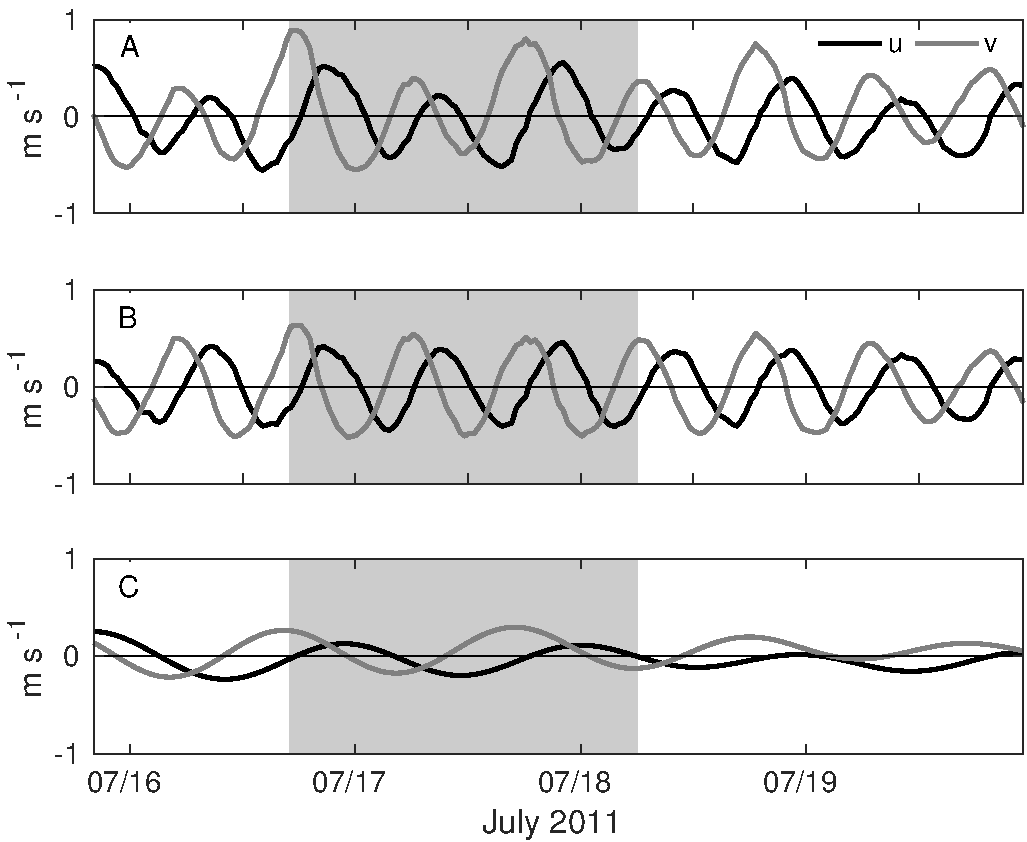
\includegraphics[width=30pc]{timeseries.pdf}
  \caption{Time-series of cross-slope ($u$) and along-slope ($v$)
    velocity components based on ADCP measurements in 30~m depth at
    position S: (a) unfiltered data, (b) highpass-filtered $M_2$ tidal
    currents, and (c) lowpass-filtered diurnal
    and subtidal currents. Period with microstructure measurements at
    position S is indicated in gray.}
  \label{tides}
\end{figure}

To decompose the observed signals into semi-diurnal and diurnal
components, we used a phase-preserving high-order filter with a cutoff
frequency of 15 hours. Comparison of the unfiltered
(Fig.\ \ref{tides}a) and highpass-filtered semi-diurnal velocities
(Fig.\ \ref{tides}b) clearly shows that the currents at our study site
were dominated by a regular $M_2$ tide with an amplitude of
approximately 0.5 m~s$^{-1}$, with slightly more energy in the
along-slope direction. This tidal constituent explains approximately
83\% of the total variance of the signal. The diurnal signal
(Fig.\ \ref{tides}c) is substantially weaker, and shows a clear trend
for both decreasing magnitude and and increasing frequency during the
observational period. Pure tidal motions are unlikely to exhibit such
variability on a time scale of only a few days, suggesting that the
observed signal is a mixture of near-inertial motions, which may
quickly vary in time due to their direct dependence on the wind
forcing, and different diurnal tidal constituents.

It is worth noting that a detailed tidal model of the East China Sea
by \cite{Baoetal2000} yields a velocity amplitude of approximately
0.5~m~s$^{-1}$ for the $M_2$ component at position S, in good
agreement with our data. For the diurnal $K_1$ tide, velocity amplitudes around
0.1~m~s$^{-1}$ were found, approximately twice as large as those of the
$O_1$ constituent. Our observations (see Fig.\ \ref{tides}c) suggest
that the model of \cite{Baoetal2000} slightly overestimates tidal
motions in the diurnal frequency band.

\section{Observations and model parameters}\label{observations}

\subsection{Observations}

The observations at position S have been described in detail by
\cite{Endohetal2016a}. Here, we only summarize their main findings to
provide the context for the discussion of the models results below.

Fig.\ \ref{meanprofiles} shows the averaged vertical structure of
salinity $S$, potential temperature $\theta$, potential buoyancy $b$,
and the (square of the) buoyancy frequency $N^2$, based on the average
of all profiles obtained at position S. Here, we define the buoyancy
as $b = - g (\rho_\theta-\rho_0)/\rho_0$, where $\rho_\theta$ is
potential density and $\rho_0=1000$~kg~m$^{-3}$ a constant reference
density. The figure shows that the lower part of the water column is
characterized by a nearly well-mixed BBL of more than 35~m thickness,
capped by a strongly stratified ``interior'' region with approximately
linear stratification, slightly larger than $N^2=10^{-3}$~s$^{-2}$.
Inside the BBL, the average stratification is 1-2 orders of magnitude
smaller compared to this interior region (Fig.\ \ref{meanprofiles}d).

\begin{figure}
  \noindent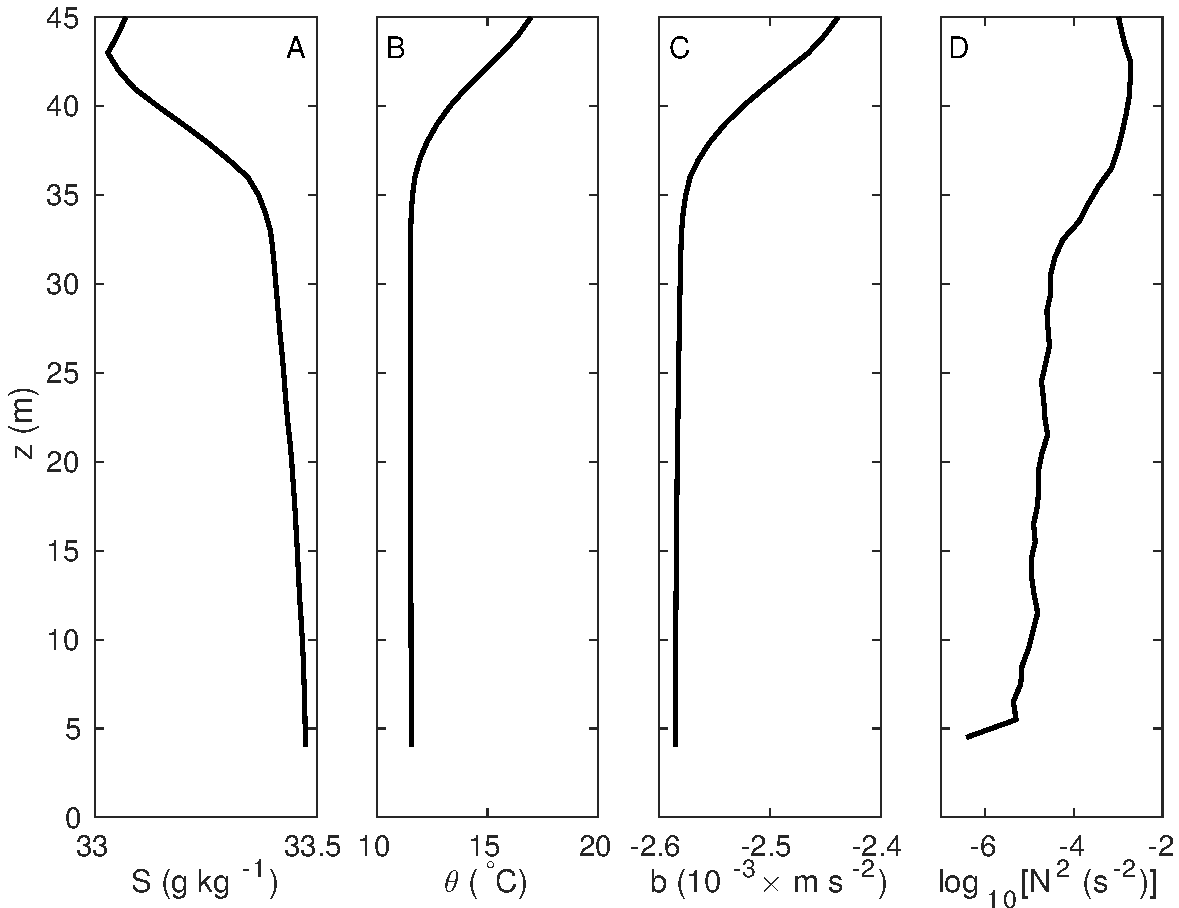
\includegraphics[width=30pc]{res_daten.pdf}
  \caption{Mean profiles of: (a) salinity, (b) potential temperature,
    (c) buoyancy, and (d) buoyancy frequency squared. Profiles are based on the 
average of all available microstructure profiles at station S (gray-shaded 
period in Fig.\ \ref{tides}).}
  \label{meanprofiles}
\end{figure}

As already discussed in the context of Fig.\ \ref{tides}, BBL
velocities are dominated by regular $M_2$ tidal motions, however, with
a significant diurnal modulation and indications for a frictional
reduction of the tidal velocities toward the bottom
(Fig.\ \ref{fielddata}a,b). Also the buoyancy anomaly
$\tilde{b}=b-\langle b \rangle$, where $ \langle b \rangle$ denotes
the tidally-averaged buoyancy shown in Fig.\ \ref{meanprofiles}c, is
characterized by a clear $M_2$ tidal variability with a $\pi/2$ phase
lag with respect to the $u$-component (Fig.\ \ref{fielddata}c). This
phase shift is expected if buoyancy variations are due to advection of
a constant cross-slope buoyancy gradient as mathematically described
by (\ref{beq}).

\begin{figure}
  \noindent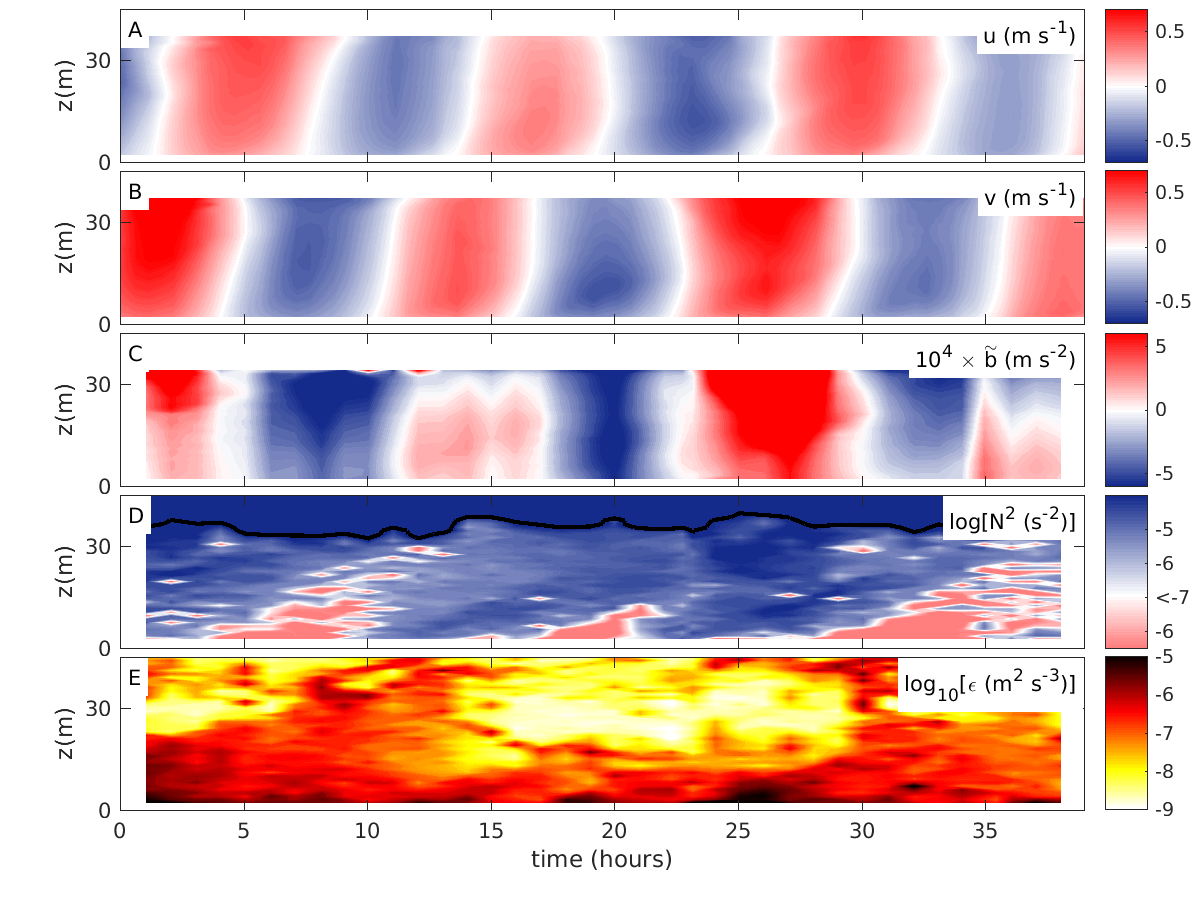
\includegraphics[width=40pc]{daten_teos10.png}
  \caption{Evolution of observed (a) cross-slope velocity, (b)
    along-slope velocity, (c) buoyancy fluctuations, (d) buoyancy
    frequency, and (e) turbulence dissipation rate. Note the special
    logarithmic color scale in (d): for $N^2 < 0$ (unstable
    stratification), the value of $| N^2 |$ is plotted in red shading,
    whereas regions with positive $N^2$ are plotted in blue
    shading. The black line indicates values of $N^2 = 10^{-3.7}$~s$^{-2}$ and 
    marks the vertical extent of the BBL. The time axis starts on 17 July 
    16:00 JST.}
  \label{fielddata}
\end{figure}

In the context of the present study, the most interesting feature in
these observations is the periodic destabilization of the lower part
of the BBL (Fig.\ \ref{fielddata}d) that \cite{Endohetal2016a} showed
to be consistent with slope-induced tidal straining as delineated in
Fig.\ \ref{sketch}. These unstable regions appear at the $M_2$ tidal
frequency, exhibit a significant vertical phase shift, and affect a
large fraction of the BBL. Beyond the key role played by the $M_2$
tidal currents in this processes a diurnal suppression of the vertical extent 
of 
the unstable regions is visible in Fig.\ \ref{fielddata}c), which should be 
kept in mind when interpreting the model results below (the diurnal signal is 
neglected in our model forcing).

Despite the dominant $M_2$ tidal forcing, the turbulence dissipation
rates shown in Fig.\ \ref{fielddata}d do not exhibit a clear tidal
signal. This is easily understood from the fact that the near-bottom
velocity vector at position S essentially rotates at the $M_2$ tidal
frequency without large modulations in magnitude (Fig.\ \ref{tides}c),
different from previous field studies in regions with more rectilinear
tides \citep[e.g.][]{Simpsonetal2002,Burchardetal2002a}. Noticeable is 
therefore 
in particular a diurnal modulation of the dissipation rate that is shown to be 
related to the vertical shear caused by the interference between diurnal and 
semidiurnal tidal currents rather than to the lateral advection of 
stratification in the upper part of the BBL \citep{Wakataetal2016a}.


\subsection{Model parameters}\label{parameters}

The solution of the system of equations in (\ref{ueq}) - (\ref{uvbBC})
depends on a number of model parameters that determine: the properties
of the rotating fluid ($f$, $N_\infty$), the slope ($\alpha$, $z_0$),
and the tidal forcing ($P_x$, $P_y$). In addition, if the transport of
suspended material is considered, the erosion parameter $\alpha_e$,
the critical shear-stress $\tau_c$, and the sinking speed $w_s$
appearing (\ref{ceq}) and (\ref{Fz}) have to be specified.

Most obvious is the choice of the Coriolis parameter ($f=7.65 \times
10^{-5}$~s$^{-1}$) and the bottom slope ($\alpha=3 \times 10^{-4}$),
which can be determined without further assumptions from the local
latitude and the echo sounding data obtained during the cruise,
respectively (see above). As the bottom roughness is not well
constrained, we chose a standard value here ($z_0=0.001$~m), and
discuss the sensitivity of our results with respect to this parameter
in Appendix B.

The determination of the time-dependent forcing functions $P_x(t)$ and
$P_y(t)$ is based on the following considerations. Firstly, we require
a purely monochromatic forcing as in (\ref{Pn}) in order to allow the
model to reach periodic conditions after an appropriate spin-up period
to be able to compute well-defined tidal averages. Secondly, in view
of the idealized nature of our model, we will focus on forcing
functions that are as simple as possible but still sufficient to
mirror all key features of the observed BBL dynamics.

With this rationale in mind, and recalling that the $M_2$ tide largely
determines the observed velocity variance at our study site, we
computed the forcing functions based on the amplitude and phase of a
pure $M_2$ tide with period $T_{M_2} = 12.42\,\text{h}$. Also, as
discussed above in the context of (\ref{omegac}), the diurnal tidal
components are close to the critical period, $T_c=22.7$~h, which is
likely to induce unphysical resonance effects in the modeled BBL.

We thus fitted a sinusoidal $M_2$ signal to the highpass-filtered
velocity data shown in Fig.\ \ref{tides}b, using the standard
least-squares fitting procedure described in \cite{EmeryThomson2001a},
however, with the following difference: the axes ratio of the tidal
ellipse was kept fixed at the value $\omega/f$ for consistency with
the model solution in (\ref{Un}). This modified fitting procedure
yields a tidal ellipse with a velocity amplitude of 0.53~m~s$^{-1}$
along the major axis, which is rotated at an angle of 107 degrees
counter-clockwise with respect to the along slope direction (see
Fig.\ \ref{fitellipse}). The analytical solution is seen to slightly
overestimate the observed ellipticity but provides otherwise a good
representation of the data.  It is worth noting that orientation and
tidal amplitude are also consistent with the $M_2$ tidal ellipse found
by \cite{Baoetal2000} near this position.

\begin{figure}
  \noindent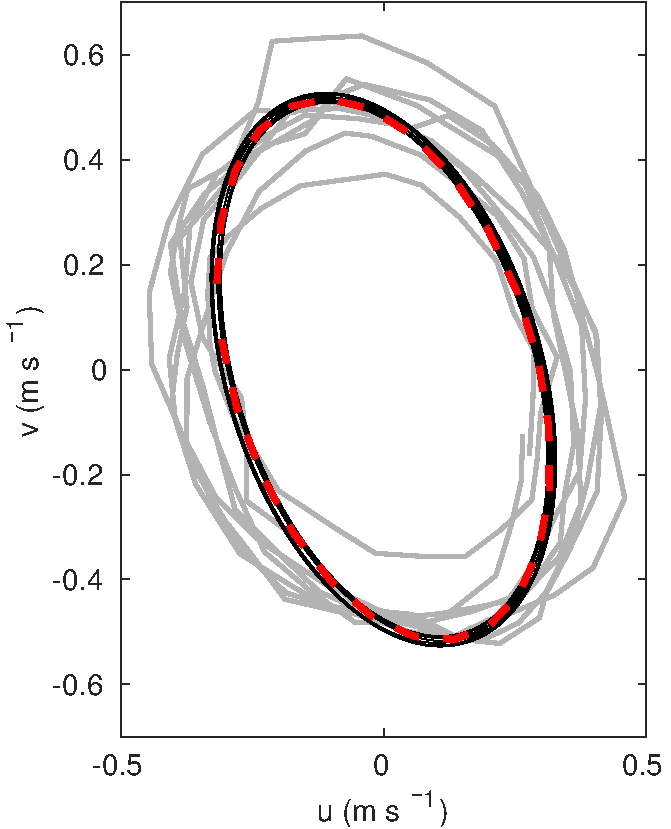
\includegraphics[width=20pc]{fitellipse.pdf}
  \caption{Highpass-filtered $M_2$ tidal currents at 30~m depth (light
    gray) and modeled velocities in the region above the BBL (black
    lines). The dashed red line indicates a fit to the data based on a
    tidal ellipse with prescribed axes ratio $\omega \slash f$.}
  \label{fitellipse}
\end{figure}

In the next step, we computed amplitude and phase of the pressure
function $P_n$ defined in (\ref{Pn}) be inverting (\ref{Un}), using
the observed velocity amplitude. Projecting the result onto the $x$-
and $y$-directions finally yields the required pressure functions
$P_x(t)$ and $P_y(t)$. As shown above, fully periodic model solutions
for this type of pressure forcing correspond to the tidal ellipse
described by (\ref{Un}) in the non-turbulent model region above the
BBL. However, numerical tests have shown that transients (mainly
inertial oscillations) generated during the abrupt start of the
simulations do not decay in this region due to the lack of any
physical damping mechanism. The problem can be strongly reduced (but
not fully eliminated) by linearly increasing the periodic pressure
forcing from zero to full amplitude over a period of 10 days. After a
spin-up period of additional 40 days, the solutions become fully
periodic inside the BBL (where transients quickly decay as a result of
viscous damping) and nearly periodic in the undamped region above the
BBL (see Fig.\ \ref{fitellipse}). As we are only interested in the
processes inside the BBL, small deviations from perfect periodicity
above the BBL are of no consequence for the following analyses.

Finally, the relevant background stratification $N_\infty$ can be
conveniently computed from the cross-slope buoyancy gradient $\partial
b / \partial x$, using the projection relation in (\ref{dbdx}). Here,
we estimate $\partial b / \partial x$ following \cite{Endohetal2016a},
who noted that buoyancy fluctuations inside the nearly well-mixed BBL
are largely determined by up- and downslope advection. Thus, for this
purpose, the buoyancy equation in (\ref{beq}) can be approximated as
\begin{equation}
  \label{badv}
  \frac{\partial b}{\partial t} = -u \frac{\partial b}{\partial x} \; ,
\end{equation}
assuming that $\partial b / \partial x$ is constant.

Similar to \cite{Endohetal2016a}, we find that $\partial b / \partial
x=2 \times 10^{-7}$~s$^{-2}$ largely explains the observed buoyancy
fluctuations due cross-slope tidal motions (see below). According to
(\ref{dbdx}), for the observed bottom slope, this value yields
$N_\infty^2 \approx 7 \times 10^{-4}$~s$^{-2}$, slightly smaller than
the measured vertical stratification above the BBL
(Fig.\ \ref{meanprofiles}d) but of the correct order of magnitude. As
pointed out by \cite{Endohetal2016a}, the relevant interior
stratification for slope-induced tidal straining is that
\emph{adjacent} to the BBL (i.e., in the interior region located at
the same depth level as the BBL at position S) rather than
\emph{above} the BBL. It is likely that the real interior
stratification adjacent to the BBL, rather than being vertically
homogeneous as assumed in our model, slightly decays with depth away
from the thermocline region.

\section{Modeling slope-induced tidal straining} \label{modelresults}

Using the periodic tidal forcing described in
section~\ref{modelproperties}, and the model parameters in
Tab.\ref{input}, we investigate in the following to which extent our
idealized model is able to reproduce the features of the observed
BBLs. For easier comparison between field data (Fig.\ \ref{fielddata})
and model results (Fig.\ \ref{modeloutcome}), time axes have been
aligned to reproduce the correct phase relationships in the $M_2$
tidal currents after the model has become periodically stationary. Due
to their periodic nature, model results are only shown for two tidal
periods for clarity.

\begin{figure}
  \noindent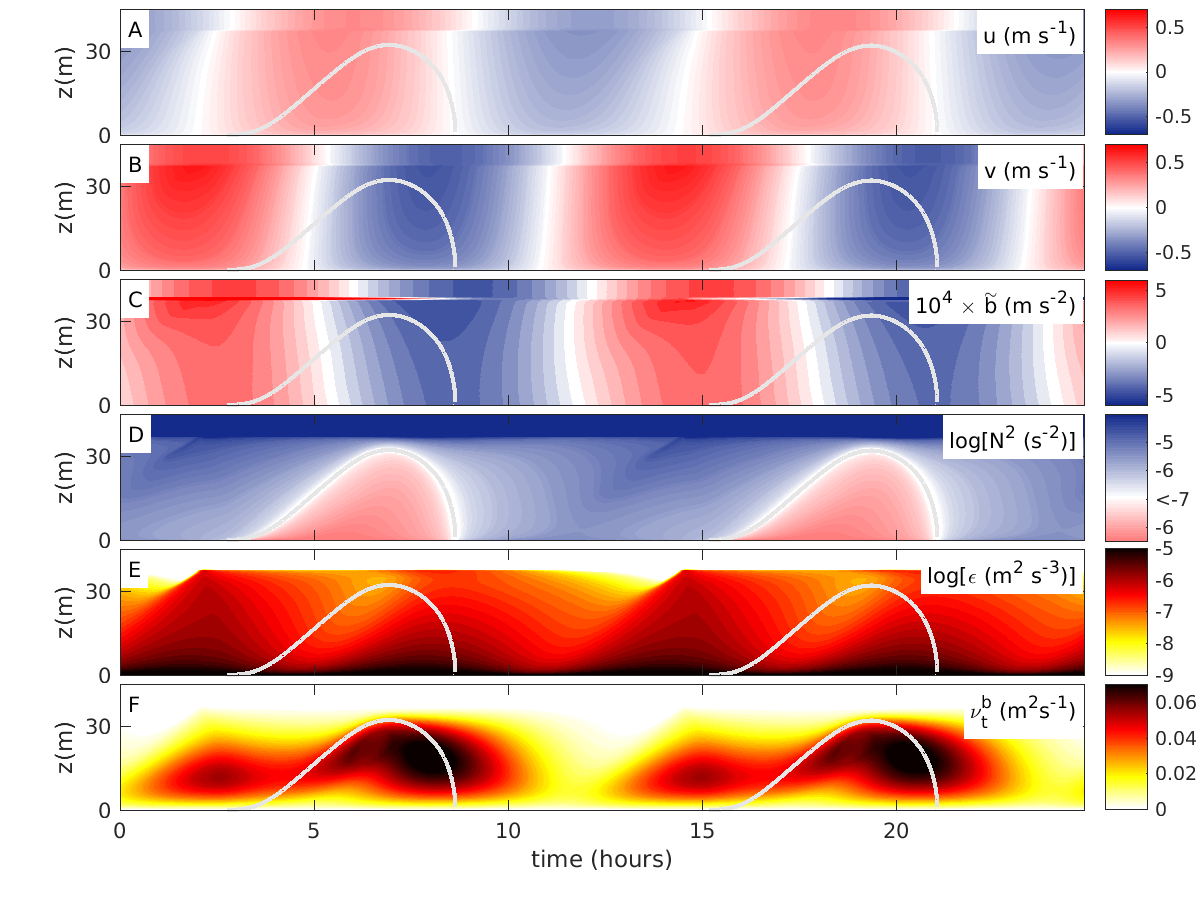
\includegraphics[width=40pc]{modeloutcome.png}
  \caption{Evolution of modeled (a) cross-slope velocity, (b)
    along-slope velocity, (c) buoyancy fluctuations, (d) buoyancy
    frequency, (e) turbulence dissipation rate, and (f) turbulent
    diffusivity. Gravitationally unstable regions are indicated by
    gray lines in all panels. Axes ranges, color scales, and time axis
    are identical to those used in Fig.\ \ref{fielddata}. }
  \label{modeloutcome}
\end{figure}

The modeled velocities (Fig.\ \ref{modeloutcome}a,b) mirror the
observed $M_2$ tidal variability with good accuracy but do not exhibit
the observed diurnal modulation, which is obviously a consequence of
neglecting the diurnal tidal constituents in our simulations. As
explained above, the diurnal signal is significant but not essential
for the process studied here.  Similar to the observations, also the
model results show clear indications for a frictional reduction of the
velocities towards the bottom, which is an essential requirement for
the development of SIPS.

Also the magnitude and phase of the tidal buoyancy fluctuations shown
in Fig.\ \ref{modeloutcome}c are in good agreement with the data,
supporting the idea that the variability in buoyancy is largely a
result of cross-slope advection as discussed above. The strong diurnal
modulation of the buoyancy fluctuations in the upper part of the BBL
found in the observations is, however, not represented by the
model, as diurnal tides are ignored in our simulations.

While the good agreement between model and data regarding the tidal
velocity and buoyancy fluctuations is largely a result of the selected
forcing variables and model parameters, the correct prediction of BBL
stratification provides a much more stringent test of the model
performance. Fig.\ \ref{modeloutcome}d shows that the model provides
an excellent representation of the evolution of BBL stratification in
at least two important aspects. First, the predicted BBL thickness is
approximately 37~m, and therefore well inside the observational range
(see Fig.\ \ref{fielddata}d). In view of the complex interplay between
slope-induced re-stratification and mixing that determines the BBL
thickness, this is a remarkable result. Second, the model is also able
to reproduce the periodic generation and destruction of stratification
(SIPS) inside the BBL, in particular regarding the occurrence of
gravitationally unstable layers during periods of upslope flow. The
observed and modeled unstable layers have a similar vertical extent
and timing but, different from the model, the observations also
exhibit a strong diurnal modulation of stratification that leads to a
suppression of the convective layer thickness during every second
instance of their occurrence (e.g., at $t \approx 20$~h in
Fig.\ \ref{fielddata}d), which cannot be reproduced in the model, of course,
again because diurnal tides are ignored.

As pointed out above, the imprint of this diurnal modulation in
stratification is also clearly visible in the observed dissipation
rates (Fig.\ \ref{fielddata}e) but, for the reasons described above,
cannot be reproduced by the model. The model does, however, correctly
predict the strong increase of the dissipation rates towards the
bottom, and the correct order of magnitude of dissipation at the
beginning and end of observation period (Fig.\ \ref{modeloutcome}e). Modeled
dissipation rates show a $M_4$ periodicity with a $M_2$ modulation
that reflects the ellipticy of the tidal currents: largest dissipation
rates are found at peaks of the $v$-component, which dominates the
$M_2$ tidal motions (see above).

While the variability in the modeled dissipation rates is therefore
mainly driven by variations in tidal forcing, the eddy diffusivities
shown in Fig.\ \ref{modeloutcome}f are also strong affected by
variations in stratification associated with SIPS. Although peaks in
dissipation rate and eddy diffusivity approximately coincide, the
latter shows a much stronger tidal asymmetry: largest diffusivities
are found during periods of upslope flow, when slope-induced tidal
straining reduces vertical stratification, or even causes regions with
negative $N^2$. We will see in the following that this modulation of
the eddy diffusivity is essential for the generation of residual
transports.



\section{Dynamics of suspended material} \label{residuals}

One of the most important implications of tidal straining is the
generation of residual currents and residual transports of dissolved
substances and suspended material. \cite{Endohetal2016a} speculated
that this process may also play an essential role for the transport of
suspended material at their study site in the East China Sea. Although
their turbidity measurements (see their Fig.\ 2i) clearly show
strongly enhanced concentrations of suspended material inside the BBL,
their data were too limited to draw any definite conclusions about
residual SPM transports. In the following, we therefore discuss a
number of idealized simulations to clarify the mechanisms and
potential implications of slope-induced tidal straining for the
residual transport of suspended material.

\subsection{Temporal variability}\label{temporal}

Our simulations are based on the SPM transport equation in (\ref{ceq})
and the simple erosion model in (\ref{Fz}). Lacking information about
sediment properties at the study site, we vary the sinking speed,
identified by \cite{schulzumlauf2016} as the key parameter
determining the transport of suspended material, over a broad range of
values. For the critical shear stress, $\tau_c$, and the erosion
parameter, $\alpha_e$, shown to be of only secondary importance by
\cite{schulzumlauf2016}, we adopt the standard values suggested by
these authors (see Tab.\ \ref{input}).

\begin{figure}
  \noindent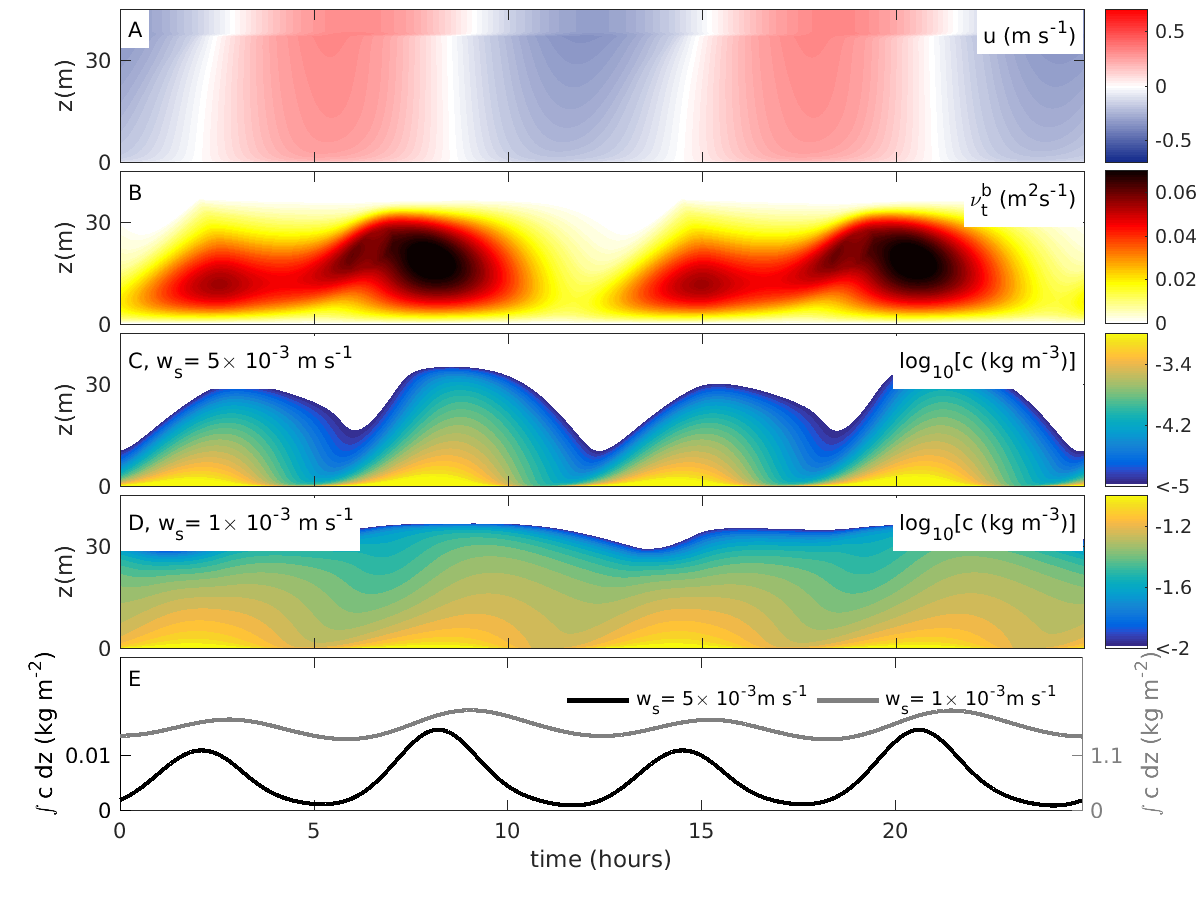
\includegraphics[width=40pc]{divc.png}
  \caption{Evolution of (a) cross-slope velocity, (b) turbulent
    diffusivity, and (c,d) SPM concentrations for two different
    settling velocities: $w_s=5 \times 10^{-3}$~m~s$^{-1}$ and $w_s=1
    \times 10^{-3}$~m~s$^{-1}$. Panel (e) shows the corresponding
    integrated SPM concentrations. Panels (a) and (b) are re-drawn
    from Fig.\ \ref{modeloutcome}a,f for better orientation.}
  \label{wsdifference}
\end{figure}

Fig.\ \ref{wsdifference}c,d reveals for two different sinking speeds
that maxima in the SPM concentrations follow maxima in the turbulence
diffusivities with a small phase shift, which mirrors the time
required to mix eroded material up into the BBL. Concentration maxima
are found when the cross-slope velocity $u$ is close to zero
(Fig.\ \ref{wsdifference}a), or, likewise, when the magnitude of the
more energetic along-slope flow component $v$ attains maximum values
(Fig.\ \ref{modeloutcome}b). Tidal asymmetries resulting from the
modulation of the turbulent diffusivity due to SIPS are clearly
evident in both local and vertically integrated SPM concentrations
(Fig.\ \ref{wsdifference}c-e). For large sinking speeds
(Fig.\ \ref{wsdifference}c), highest concentrations are found at the
end of the period with upslope flow, when turbulent diffusivities are
maximum, along-slope velocities close to their maximum negative values
($v<0$), and cross-slope velocities close to zero. Similar SPM maxima
are also found at the end of downslope flow period, however, with
significantly smaller concentrations due to the comparably smaller
turbulent diffusivities.

The strong correlation between high SPM concentrations and negative
along-slope speeds constitutes a tidal pumping mechanism that, as
discussed in more detail below, leads to a vigorous residual transport
of suspended material along the slope in the negative
$y$-direction. Tidal pumping is much less effective in the cross-slope
$x$-direction because SPM concentration maxima are associated with
minima in the magnitude of the cross-slope velocity ($u \approx
0$). Although tidal asymmetries in SPM concentrations can also be
discerned for the case with low sinking speeds
(Fig.\ \ref{wsdifference}d,e), they are less pronounced, and their
potential to trigger tidal pumping is therefore expected to weaker.

Finally, it is worth noting that the collapse of cross-slope tidal
pumping mentioned above is qualitatively different from the
non-rotating case investigated by \cite{schulzumlauf2016}. Although
their simulations showed similar tidal asymmetries with highest
turbulent diffusivities and SPM concentrations observed during periods
of upslope flow, these maxima occurred earlier compared to the rotating
case. This is easily understood from the fact that in the non-rotating
case the $v$-component, dominating BBL turbulence in our case, is
lacking, and highest diffusivities are thus observed significantly
before the upslope flow reversal. In the non-rotating case, high SPM
concentrations are therefore correlated with significant upslope
velocities ($u>0$), resulting in an effective upslope pumping of
suspended material.


\subsection{Residual transports}\label{residualtransports}
The residual transports of suspended material in the cross-slope and
along-slope directions are defined as
\begin{equation}
  \label{FxFy}
  F_x = \langle u c \rangle - \langle c \rangle w_s \sin \alpha \; , \quad
  F_y = \langle v c \rangle \; ,  
\end{equation}
where the angular brackets denote the tidal average. The second term
in the cross-slope flux $F_x$ represents the small downslope motion of
vertically sinking material near a sloping
bottom. \cite{schulzumlauf2016} showed that this term is generally
negligible for small slopes ($\alpha \ll 1$), and therefore will be
ignored in the following.

\cite{schulzumlauf2016} also pointed out that the fluxes defined in
(\ref{FxFy}) are of limited use for the analysis of the tidal
transport mechanisms due to their direct dependency on the SPM
concentrations. Instead, they suggested to normalize the SPM fluxes
with the concentrations, which removes this dependency:
\begin{equation}
 \label{ucvc}
 \begin{array}{rcl}
 u_c &=& \displaystyle 
            \frac{\langle u c \rangle}{\langle c \rangle} 
         =  \langle u \rangle + \frac{\langle \tilde{u} \tilde{c} 
\rangle}{\langle c \rangle} \; , \\[5mm]
 v_c &=& \displaystyle
           \frac{\langle v c \rangle}{\langle c \rangle} 
         =  \langle v \rangle + \frac{\langle \tilde{v} \tilde{c} 
\rangle}{\langle c \rangle} \; .
 \end{array}
\end{equation}
The normalized velocities $u_c$ and $v_c$ are recognized as the
effective velocities at which SPM is transported across and along the
slope during a tidal cycle. In the second step in (\ref{ucvc}), we
have further decomposed all quantities into tidal averages and
fluctuations (denoted by the tilde), revealing that the transport
velocities are the sum of the residual velocities and correlation
terms representing the effect of tidal pumping.

\begin{figure}
  \noindent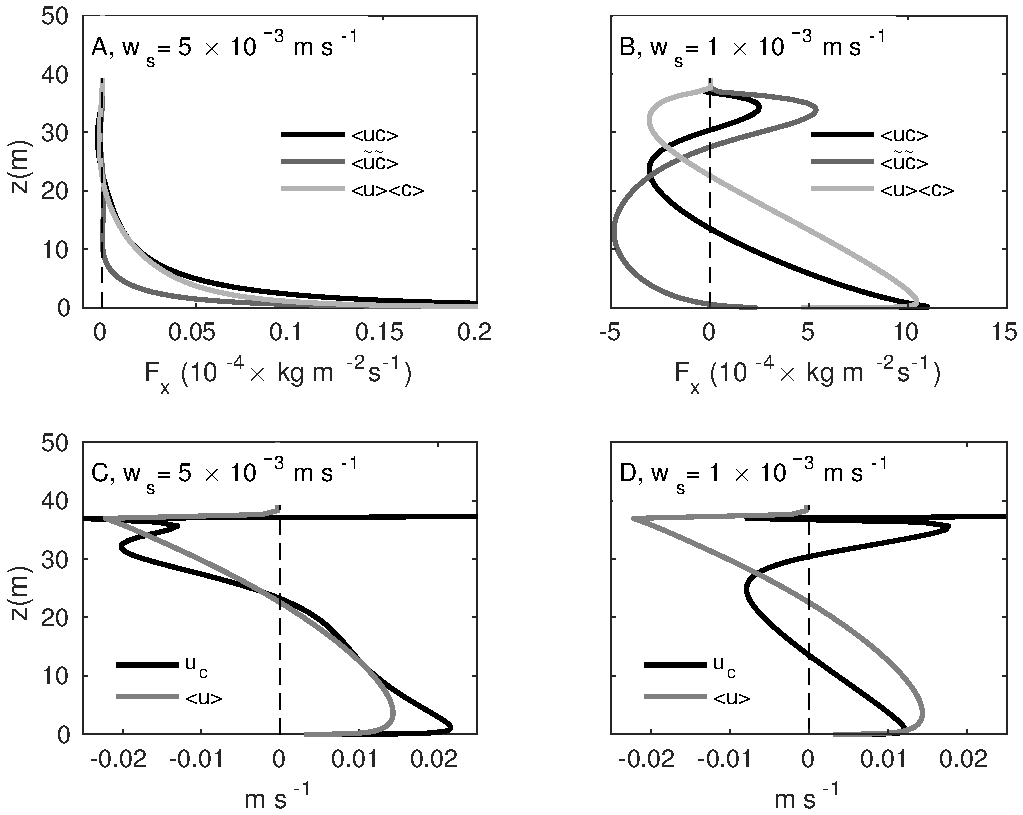
\includegraphics[width=40pc]{restrans.pdf}
  \caption{Residual cross-slope fluxes of suspended material for
    settling velocities (a) $w_s = 5 \times 10^{-3}$~m~s$^{-1}$ and
    (b) $w_s = 1 \times 10^{-3}$~m~s$^{-1}$ with contributions from
    the residual currents and tidal pumping as indicated. Panels (c)
    and (d) show the corresponding effective transport velocities
    defined in (\ref{ucvc}). Note the different axes ranges. }
  \label{residualu}
  
\end{figure}
Figs.\ \ref{residualu} and \ref{residualv} compare cross-slope and
along-slope SPM fluxes for the two sinking speeds shown in
Fig.\ \ref{wsdifference}c,d. As already speculated in section
\ref{temporal}, for the larger sinking speed the contribution of tidal
pumping to the total cross-slope flux is small due to the fact that
high SPM concentrations generally co-occur with negligible cross-slope
speeds (Fig. \ref{residualu}a). This is confirmed by
Fig.\ \ref{residualu}c, showing that the transport velocity $u_c$ is
of the same order of magnitude as the residual current $\langle u
\rangle$. Different from the non-rotating case investigated by
\cite{schulzumlauf2016}, tidal pumping is therefore not the
dominating process in this example. This is also true for the case
with a small sinking speed (Fig. \ref{residualu}b,d), which is,
however, further complicated by the fact that the contributions of the
residual current and tidal pumping may point into different
directions.

\begin{figure}
  \noindent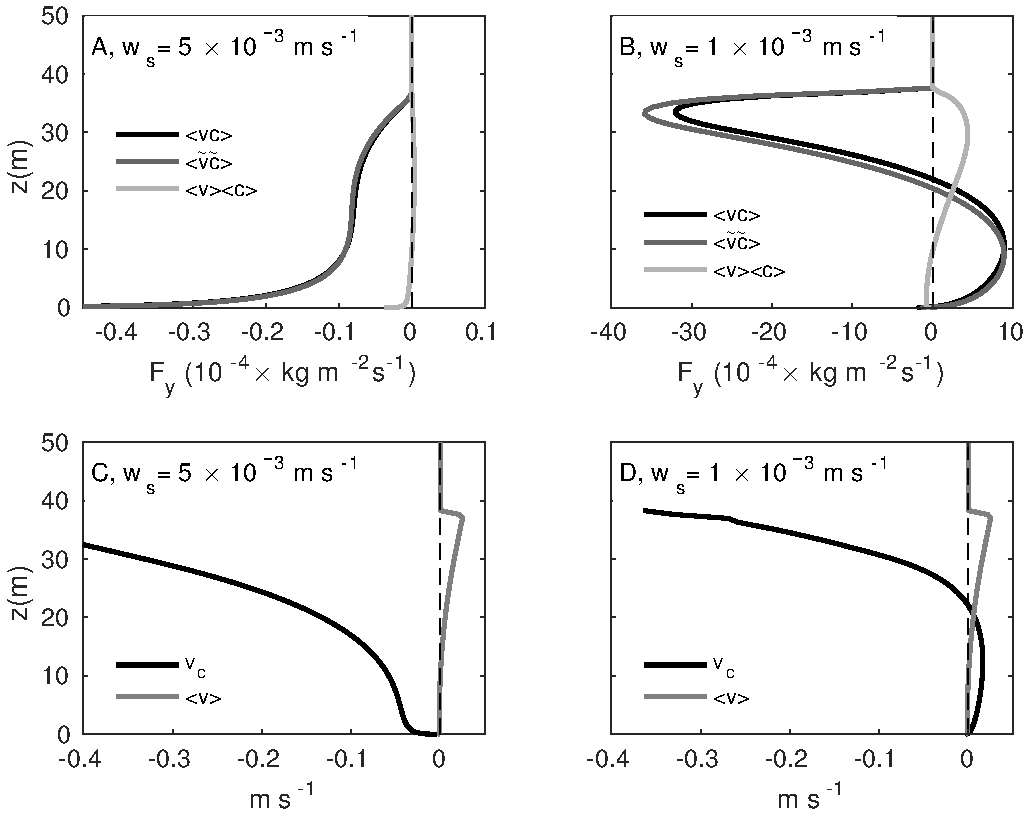
\includegraphics[width=40pc]{restransv.pdf}
  \caption{As in Fig.\ \ref{residualu}, but now for the along-slope
    SPM fluxes and transport velocities. Note that the axes ranges are
    different from Fig.\ \ref{residualu}.}
  \label{residualv}
\end{figure}

The situation changes completely if the along-slope fluxes are
considered. Fig.\ \ref{residualv}a,b shows that for both sinking
speeds tidal pumping provides the overwhelming contribution to the net
SPM fluxes. The strong correlation between large SPM concentrations
and negative along-slope velocities for the case with a large sinking
speed (see section \ref{temporal}) induces a residual flux of
suspended material in the negative $y$-direction that is almost one
order of magnitude larger than the corresponding cross-slope flux
(Fig.\ \ref{residualu}a). The effectiveness of tidal pumping in this
case is corroborated by Fig.\ \ref{residualv}c, showing that the
contribution of the residual current to the effective transport
velocity $v_c$ is generally negligible. Typical transport velocities
in the lower part of the BBL, where SPM concentrations are high, are
of the order of $0.1$~m~s$^{-1}$, suggesting that suspended material
is transported approximately 5~km along the slope during one tidal
cycle.

Particularly notable is the two-layer structure determining the
along-slope SPM transport for the case with a low sinking speed
(Fig.\ \ref{residualv}b), which may be explained as follows. Comparing
the along-slope velocities in Fig.\ \ref{modeloutcome}b and the SPM
concentrations in Fig.\ \ref{wsdifference}d shows that during periods
of positive along-slope flow, near-bottom SPM concentrations are
highest because stable stratification prevents resuspended material to
be diluted by mixing across a larger fraction of the BBL. The opposite
is the case for periods with negative along-slope flow. Here, SPM is
mixed up high into the BBL, because mixing is not suppressed by stable
stratification any more. The net effect of the resulting correlations
is a positive along-slope transport near the bottom, and a negative
transport in the upper part of the BBL.


\subsection{Variable sinking speed and stratification}
To quantify the variability of SPM transport across a larger parameter
space, it is useful to introduce the normalized integrated fluxes,
\begin{equation}
  \label{ucint}
  U_c = \frac{ \int \langle uc \rangle dz}{\int \langle c \rangle dz}
  \; , \quad V_c = \frac{\int \langle vc \rangle dz}{\int \langle c
    \rangle dz} \; .
\end{equation}
Analogous to the vertically variable transport velocities $u_c$ and
$v_c$, the vertically integrated expressions in (\ref{ucint}) define
bulk measures for the residual velocities at which SPM is transported
across and along the slope, respectively \citep{schulzumlauf2016}.

\begin{figure}
  \noindent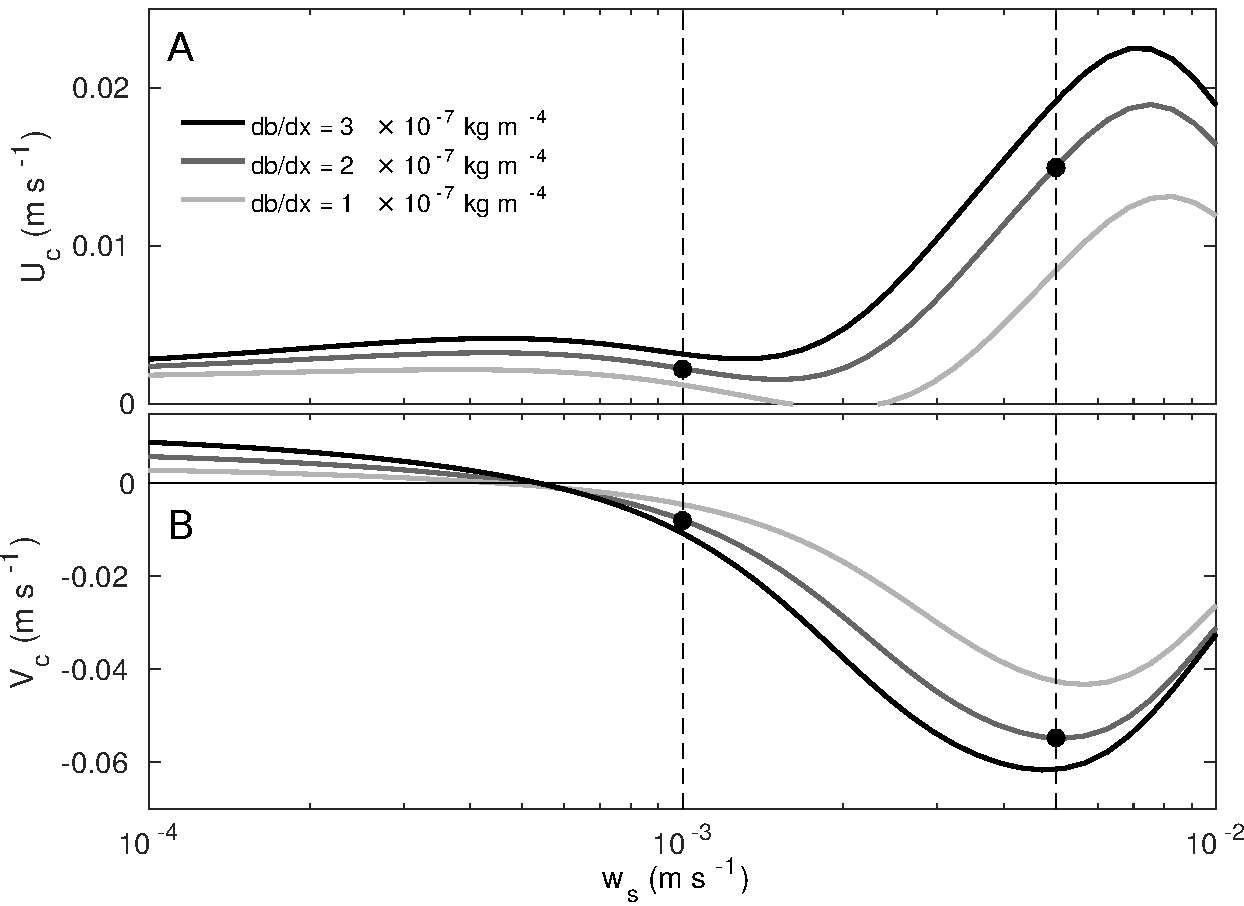
\includegraphics[width=30pc]{wsvariation.pdf}
  \caption{Distribution of (a) cross-slope and (b) along-slope
    transport velocities, $U_c$ and $V_c$, for variable settling
    velocities and cross-slope buoyancy gradients (all other
    parameters as in Tab.\ \ref{input}).  Dashed vertical lines
    indicate the standard cases of small and large settling velocities
    discussed in the context of
    Fig.\ \ref{wsdifference}.}\label{wsvariation}
\end{figure}

In Fig.\ \ref{wsvariation}, the distribution of $U_c$ and $V_c$ for
varying settling velocities is displayed.  As already discussed in
section \ref{residualtransports}, the cross-slope sediment flux is
largely determined by the contribution of the residual current,
$\langle u \rangle \langle c \rangle$, which is directed upslope near
the bottom and downslope in the upper part of the BBL. The
contribution of tidal pumping is either relatively small (for large
sinking speeds, see Fig.\ \ref{residualu}a,c), or even counteracts the
contribution of the residual current (for small sinking speeds, see
Fig.\ \ref{residualu}b,d). The local maximum in $U_c$ for $w_s \approx
7 \times 10^{-3}$~m~s$^{-1}$ (Fig.\ \ref{wsvariation}a) can thus be
explained as follows. For settling velocities higher than this optimal
value, suspended matter remains inside a thin near-bottom layer, where
flow velocities are strongly reduced due to frictional effects. SPM
transport is not efficient in this case. Material that exhibits
settling velocities smaller than the optimal value is more
homogeneously distributed across the BBL, implying that the
near-bottom upslope transport is partly compensated by a downslope
transport in the upper part of the BBL.  The local minimum, visible
Fig.\ \ref{wsvariation}a for sinking speeds slightly larger than
$w_s=10^{-3}$~m~s$^{-1}$, originates from the effect of tidal pumping,
opposing the contribution of the residual current for material with
small settling velocities (see Fig.\ \ref{residualu}b). It is
remarkable that for virtually all settling velocities investigated
here, the transport is directed upslope, similar to the non-rotating
case studied by \cite{schulzumlauf2016}.

Different from the cross-slope transport of suspended material, the
along-slope transport is mainly determined by tidal pumping
(Fig.\ \ref{residualv}). In this case, $V_c$ reaches a local minimum
(maximum negative transport rates) near $w_s \approx 5 \times
10^{-3}$~m~s$^{-1}$. This optimum value is also marked in
Fig.\ \ref{wsvariation}, and corresponds to the case of large sinking
speed discussed in the previous sections. The maximum in the transport
rate for this value of the sinking speed is shaped by two competing
effects. For settling velocities larger than the optimum value,
suspended material is largely located inside the thin frictional
near-bottom layer, where tidal pumping is not effective and $V_c$ thus
decreases. For material sinking slower than the optimal value, the
negative near-bottom transport is partly compensated by an opposing
transport in the upper part of the BBL (see example in
Fig.\ \ref{wsvariation}b). If sinking speeds are small enough, this
effect may even cause a reversal of the transport direction
(Fig.\ \ref{wsvariation}b). Comparing the magnitudes of $U_c$ and
$V_c$ in Fig.\ \ref{wsvariation}, it is evident that along-slope tidal
pumping results in a factor of 2-3 larger transport velocities
compared to the cross-slope direction.

Finally, it is worth noting that Fig.\ \ref{wsvariation} also reveals
that stronger background stratification enhances the SPM transport
mechanisms in both the cross-slope and along-slope directions. This is
little surprising, however, as stratification is one of the
prerequisites for slope-induced tidal straining and pumping. The
existence of an optimal settling velocity for up-slope transport, and
the observed dependency on background stratification, are in agreement
with the findings of \cite{schulzumlauf2016} for the non-rotating
case.



\subsection{Rotational effects}

According to (\ref{Un}) and (\ref{Us}), the shape of the tidal ellipse
is determined by the Coriolis parameter, which is therefore likely to
have an important impact on tidal straining and SPM transport. In the
following, we investigate this effect in a series of simulations with
varying latitude (varying Coriolis parameter), leaving all other
parameters as in Tab.\ \ref{input}. For the sinking speed, we assume
$w_s=5 \times 10^{-4}$~m~s$^{-1}$, corresponding to the optimal value
for along-slope tidal pumping identified in the previous section.

We consider two special cases for the pressure forcing in
(\ref{Pn}). In the first case, we assume that the pressure force is
directed exactly in the cross-slope direction ($P_x \neq 0$, $P_y=0$),
whereas in the second case the forcing is purely along-slope ($P_x =
0$, $P_y \neq 0$). Using the analytical solution in (\ref{Un}), we
adjust the pressure force $P$ for each case exactly such that the
velocity amplitude in the direction of the forcing remains constant at
a value of 0.5~m~s$^{-1}$. This results in a tidal ellipse with the
(constant) major axes oriented parallel to the pressure force (i.e.,
either cross-slope or along-slope), and the minor axes increasing in
magnitude with increasing Coriolis parameter. The latter is varied by
changing the latitude from 20$^\circ$~N to 60$^\circ$~N at 10$^\circ$
intervals, corresponding to axes ratios between 0.35 and 0.89 for the
tidal ellipses.  Using (\ref{omegac}), it is easy to show that for the
parameters in Tab.\ \ref{input}, BBL resonance and the transition to
super-critical slopes \citep[see][]{schulzumlauf2016} occur at a
latitude of approximately 75$^\circ$~N. The range of latitudes used
here guarantees that BBL resonance does not affect the results.

\begin{figure}
  \noindent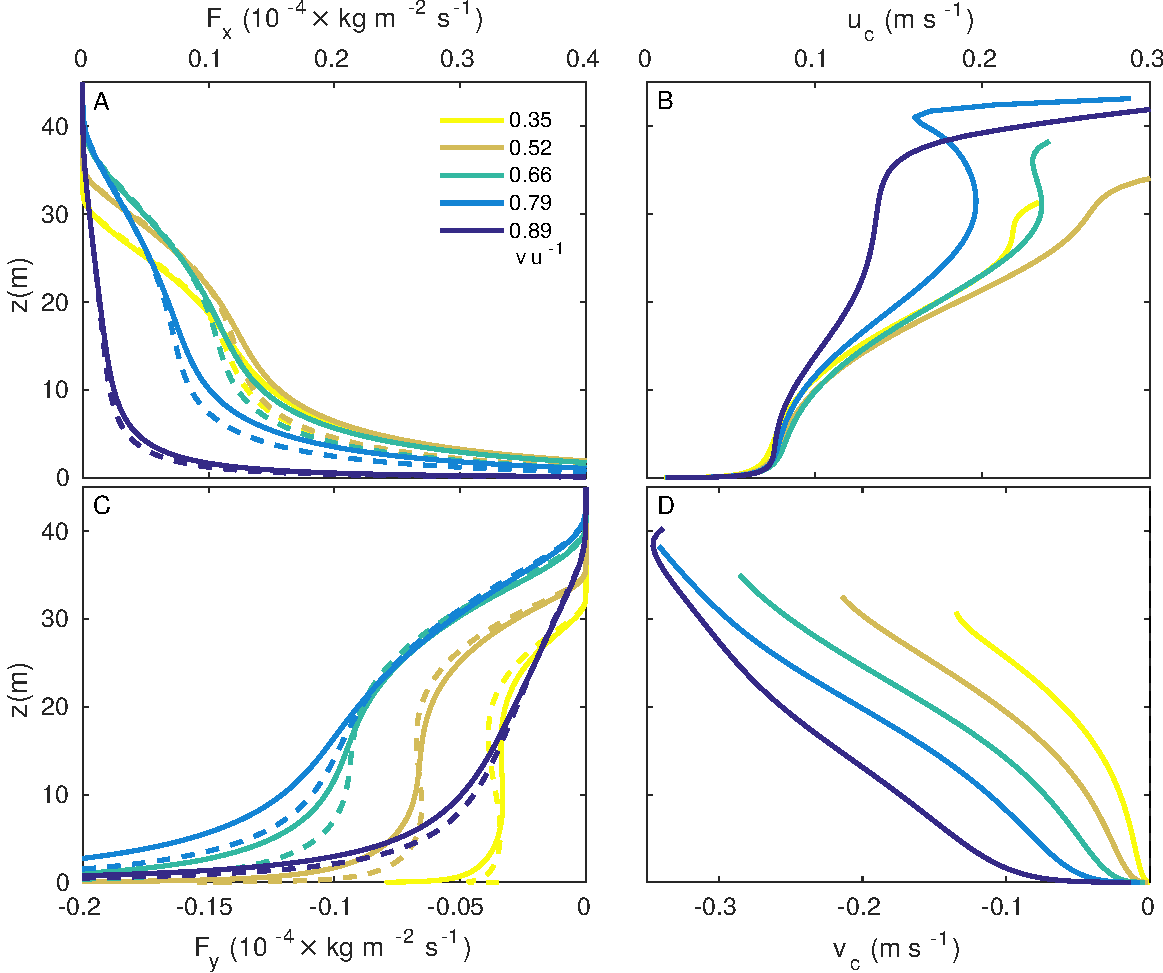
\includegraphics[width=30pc]{coriolis.pdf}
  \caption{Profiles of (a) cross-slope and (c) along-slope SPM flux,
    and (b) cross-slope and (d) along-slope transport velocity for a
    range of latitudes between 20$^\circ$~N and 60$^\circ$~N (at
    10$^\circ$ intervals).  The pressure forcing is purely cross-slope
    ($P_y=0$), and the amplitude of the cross-slope tidal velocity
    fluctuations in the region above the BBL is $u=0.5$~m~s$^{-1}$ for
    all cases. The amplitude of the corresponding along-slope
    component $v$ increases with latitude as indicated.  Dashed lines
    in (a) and (c) show the contribution of tidal pumping to the
    overall SPM flux.}
  \label{coriolis}
\end{figure}

The case with pure cross-slope forcing ($P_y=0$) includes the
non-rotational case ($f=0$, $v=0$) investigated in detail by
\cite{schulzumlauf2016}. As pointed out by these authors, the
turbulent diffusivities show in this case a clear $M_4$ signal that
exhibits a $M_2$ modulation due to SIPS (higher diffusivities are
observed during periods with upslope flow). These tidal asymmetries
trigger an efficient tidal pumping mechanism that transports suspended
material in the upslope direction. Fig.\ \ref{coriolis}a,b shows that
this mechanism remains essentially unchanged for latitudes up to
approximately 40$^\circ$~N, corresponding to a axis ratio of 0.66 for
the tidal ellipse. While the BBL thickness significantly increases
over this range of latitudes, SPM fluxes and transport velocities
exhibit only small changes in the lowest 20~m of the BBL, where most
of the suspended material is located and therefore most of the
transport occurs. Quite differently, the along-slope SPM transport,
vanishing for $f=0$, quickly increases for $f>0$ as a result of the
same tidal pumping mechanisms described in detail in sections
\ref{temporal} and \ref{residualtransports} (see
Fig.\ \ref{coriolis}c,d).

\begin{figure}
  \noindent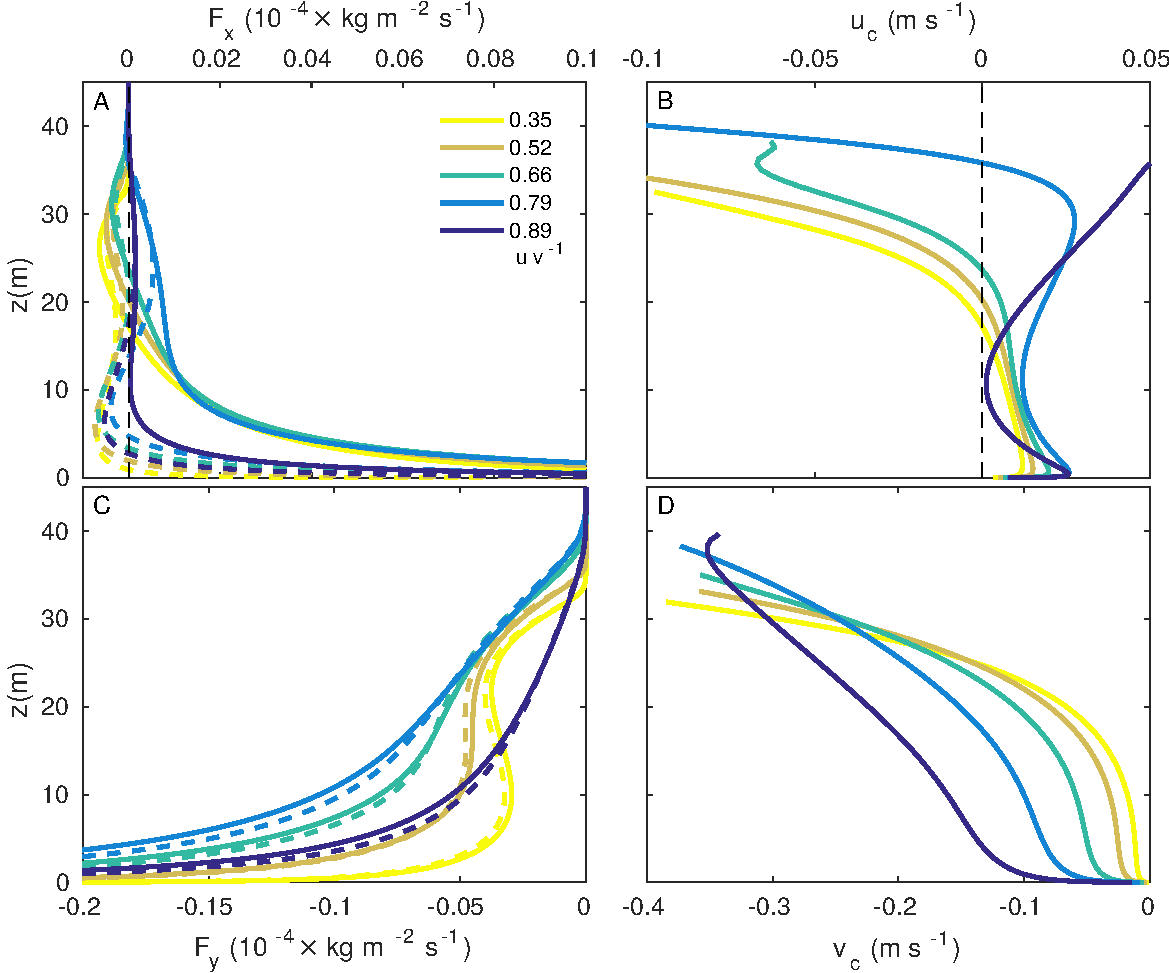
\includegraphics[width=30pc]{coriolis2.pdf}
  \caption{As in Fig.\ \ref{coriolis}, but now for along-slope
    pressure forcing ($P_x=0$), and constant amplitude of the
    along-slope tidal velocity fluctuations ($v=0.5$~m~s$^{-1}$).}
  \label{coriolis2}
\end{figure}

For higher latitudes, the tidal ellipses gradually approach a circular
shape, implying that the magnitude of the rotating velocity vector
changes only slightly during a tidal cycle. As consequence, the
turbulent diffusvity and the bottom stress (both important for SPM
erosion) show a transition from a pronounced $M_4$ variability with
two maxima during a tidal cycle towards a weak $M_2$ modulation with a
single maximum during periods with upslope flow. Considerably less
material is eroded during this single maximum compared to the cases
with smaller rotation rates, and SPM concentrations strongly
decrease. Therefore, although tidal pumping is still active or even
increasing in the along-slope direction (see Fig.\ \ref{coriolis}d),
the total SPM fluxes collapse for high latitudes
(Fig.\ \ref{coriolis}a,c).

In our second series of simulations, we assume that the tidal pressure
force is directed exactly along the slope ($P_x=0$). Different from
the case with cross-slope forcing, both the cross-slope and the
along-slope SPM fluxes vanish in the limit $f \rightarrow 0$ for
symmetry reasons. For increasing latitudes, a weak upslope transport
develops, which, similar to the example in section
\ref{residualtransports}, is driven by the residual flow rather than
by tidal pumping (Fig.\ \ref{coriolis2}a,b). The weak transport rates
in the cross-slope direction are strongly contrasted by the vigorous
along-slope tidal pumping mechanism that quickly develops for
increasing $f$ (Fig.\ \ref{coriolis2}c,d). The mechanisms are analogous
to the example discussed in the previous sections (see
Fig.\ \ref{residualv}a,c), which was also characterized by a dominant
along-slope flow component. For the highest latitudes, however, both
the cross-slope and along-slope transports collapse again due to
decreasing concentrations of suspended material. The reasons are
identical to those discussed above.